% Technical report: FastSpeech 2 for English (Svarah) and Telugu (IndicTTS)
% Build (from this folder):  xelatex Technical_Report.tex   (run twice)
% Needs the Nirmala UI font (ships with Windows) for the Telugu text.
\documentclass[11pt,a4paper]{article}
\usepackage{fontspec}
\usepackage[margin=2.0cm]{geometry}
\usepackage{graphicx,booktabs,xcolor,caption,subcaption,enumitem,tabularx,float,array,longtable,multirow}
\usepackage{tikz}
\usetikzlibrary{positioning,arrows.meta,decorations.pathreplacing}
\usepackage[hidelinks]{hyperref}
\setmainfont{Cambria}
\setmonofont{Consolas}[Scale=0.86]
\newfontfamily\te[Script=Telugu]{Nirmala UI}
\newcommand{\tel}[1]{{\te #1}}
\newcommand{\code}[1]{\texttt{#1}}
\graphicspath{{../Results/}}
\setlist{itemsep=1pt,topsep=3pt}
\captionsetup{font=small,labelfont=bf}
\setlength{\parskip}{3pt}
\renewcommand{\arraystretch}{1.12}
\emergencystretch=2em

\title{FastSpeech 2 for Indian-accented English (Svarah) and Telugu (IndicTTS)\\[3pt]\large Technical report}
\author{Simhaa T.\,T.}
\date{November 2026}

\begin{document}
\maketitle

% =====================================================================
\section{Summary}
A text-to-speech (TTS) model turns written text into speech. I trained two FastSpeech 2 TTS models from scratch
with the same architecture and recipe, one for English and one for Telugu. The English model learnt from 4.6\,h
of the Svarah corpus of Indian-accented English, using 99 of its 117 speakers. The Telugu model learnt from 4.1\,h
of one male voice in the IndicTTS Telugu corpus. Each language also kept about 1\,h of separate validation audio
(0.82\,h for Telugu after trimming silence) that shares no clip with training. As an extra experiment, I
fine-tuned a second English model from a public model trained on LJSpeech, an American English corpus. The code
starts from the open-source ming024 implementation of FastSpeech 2, and Section~\ref{sec:changes} lists every
change. Section~\ref{sec:background} explains how the system works for readers new to speech synthesis.

The English model speaks all five of its test sentences understandably. I do not speak Telugu, so a Telugu speech
recogniser (an automatic transcription model) judged that audio: it got 4.7\% of the characters wrong on
synthesised Telugu against 3.4\% on real Telugu speech, while the English recogniser got 10.0\% wrong against
6.4\%. The Telugu model comes out closer to real speech on every measure I took. On 80 validation sentences, the
Telugu model's predicted phone durations correlate with the real ones at $r = 0.85$ (English: 0.61), and its pitch
at $r = 0.75$ (English: 0.43). The English spectrograms (the model's picture of the sound) change only 63\% as
much from one 11.6\,ms frame to the next as real speech does, against 88\% for Telugu. This over-smoothing matches
what the English audio sounds like: the words come out mumbled, as if swallowed. Replacing the model's predicted
pitch and loudness with the real values brought the spectrograms 9\% (English) and 20\% (Telugu) closer to real
speech, while the real phone durations changed almost nothing. Even with timing, pitch and loudness all taken
from the recording, English stays further from real speech than Telugu, so the mumbling comes from the decoder,
the part of the model that draws the spectrogram, not from the timing. Validation loss stopped improving early in
both languages, at step 14,000 for English and 12,000 for Telugu out of 60,000. Fine-tuning from LJSpeech gave
slightly better English spectrograms but worse pitch and loudness, and no gain overall.

% =====================================================================
\section{How the system works}
\label{sec:background}
This section explains the parts of a text-to-speech (TTS) system for readers new to speech. Figure~\ref{fig:pipeline}
shows the whole path from text to audio, and Table~\ref{tab:terms} defines the measures the later sections use.

\begin{figure}[H]\centering
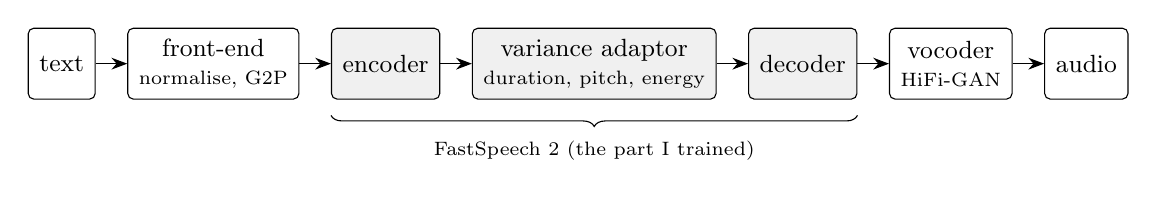
\begin{tikzpicture}[
  box/.style={draw, rounded corners=2pt, align=center, font=\small, inner sep=4pt, minimum height=9mm},
  model/.style={box, fill=black!6},
  lab/.style={font=\scriptsize, align=center},
  arr/.style={-{Stealth[length=2mm]}}]
\node[box] (text) {text};
\node[box, right=4mm of text] (fe) {front-end\\[-1pt]{\scriptsize normalise, G2P}};
\node[model, right=4mm of fe] (enc) {encoder};
\node[model, right=4mm of enc] (va) {variance adaptor\\[-1pt]{\scriptsize duration, pitch, energy}};
\node[model, right=4mm of va] (dec) {decoder};
\node[box, right=4mm of dec] (voc) {vocoder\\[-1pt]{\scriptsize HiFi-GAN}};
\node[box, right=4mm of voc] (wav) {audio};
\draw[arr] (text) -- (fe);
\draw[arr] (fe) -- (enc);
\draw[arr] (enc) -- (va);
\draw[arr] (va) -- (dec);
\draw[arr] (dec) -- (voc);
\draw[arr] (voc) -- (wav);
\draw[decorate, decoration={brace, mirror, amplitude=4pt}] ([yshift=-2mm]enc.south west) -- ([yshift=-2mm]dec.south east)
  node[midway, below=2mm, font=\scriptsize] {FastSpeech 2 (the part I trained)};
\end{tikzpicture}
\caption{From text to audio. The front-end turns text into phones; the encoder gives one vector per phone; the
variance adaptor predicts each phone's duration, pitch and energy and stretches the sequence to one vector per
frame; the decoder turns the frames into a mel spectrogram; the vocoder turns that into a waveform. The shaded
blocks form FastSpeech 2. The front-end is rules and dictionaries, and the vocoder a separate pretrained network.}
\label{fig:pipeline}
\end{figure}

\paragraph{Text to phones.} The front-end first writes the text out as it is spoken: numbers, dates and times
become words. A grapheme-to-phoneme (G2P) step then turns each word into \emph{phones}, the individual sounds of
the language (also called phonemes). English phones use ARPAbet, the symbol set of the CMU pronouncing dictionary,
where a digit after a vowel marks stress (1 primary, 2 secondary, 0 none): ``conduct'' as a noun is
\code{K AA1 N D AH0 K T}. Telugu uses its own phone set (Section~\ref{sec:te-frontend}).

\paragraph{What the model outputs.} FastSpeech 2 does not output audio. It outputs a \emph{mel spectrogram}: a grid
with time on one axis and 80 frequency bands on the other, each cell holding the loudness of that band, on a log
scale. Each column, called a \emph{frame}, covers 11.6\,ms. The bands follow the mel scale, which spaces them the way
human hearing does: narrow at low frequencies and wide at high ones. A second network, the \emph{vocoder}, turns the
mel spectrogram into a waveform. I used a pretrained HiFi-GAN vocoder and did not train it.

\paragraph{Inside FastSpeech 2.} The \emph{encoder} reads the phone sequence and gives one vector per phone. The
\emph{variance adaptor} then predicts three things for each phone: its \emph{duration} (how many frames it lasts),
its \emph{pitch} (the fundamental frequency F0 in Hz, heard as how high the voice is) and its \emph{energy} (how
loud it is). Together, timing, pitch and loudness are called \emph{prosody}. The \emph{length regulator} repeats each
phone's vector once per frame of its duration, and the \emph{decoder} turns that frame sequence into the mel
spectrogram. Because every phone gets an explicit duration, the model cannot skip or repeat words, and it produces
all frames at once instead of one after another, which makes it fast.

\paragraph{What training needs.} To learn durations, the model needs the true duration of every phone in every
training clip. A \emph{forced aligner} finds them: given the audio and its transcript, it marks where each phone
starts and ends. I used the Montreal Forced Aligner (MFA), which writes these boundaries to TextGrid files. The
true pitch and energy come from the recordings. In training the model receives the true durations, pitch and
energy and learns to predict them; when it synthesises new text, it uses its own predictions.

\paragraph{Starting point.} I built on \code{ming024/FastSpeech2}, a widely used open-source PyTorch version of
FastSpeech 2 by the GitHub user ming024. It comes with a model trained on LJSpeech, 24\,h of one American woman
reading books. Besides training from random weights, I ran one \emph{ablation}, an extra experiment that changes one
thing to measure its effect: an English model that starts from the LJSpeech weights instead (\emph{fine-tuning}).

\begin{table}[t]\centering\small
\caption{Measures used in this report.}
\label{tab:terms}
\begin{tabularx}{\linewidth}{@{}lX@{}}
\toprule
Validation loss & The training objective on held-out clips the model never trains on: mean absolute error (L1)
between generated and real mel spectrograms, plus mean squared error (MSE) between predicted and true log
duration, standardised pitch and standardised energy. Lower is better. \\
CER, WER & Character and word error rate: a speech recogniser transcribes the audio, and the rate counts the
inserted, deleted and substituted characters (or words) against the true text, as a percentage of its length.
Lower means more intelligible. \\
Correlation $r$ & Pearson correlation between predicted and real values within an utterance: 1 means they rise and
fall together, 0 means no relation. \\
Spread ratio & The standard deviation of the predictions within an utterance divided by that of the real values;
below 1 means flatter than real speech. \\
Flux, global variance & How much a mel spectrogram changes from one frame to the next (flux) and how much each band
varies over the utterance (global variance), each as generated / real. Below 1 means a smoother, more blurred
spectrogram than real speech. \\
MCD & Mel-cepstral distortion: the distance in dB between a generated and a real spectrogram of the same sentence.
Lower is closer. \\
F0 error (cents) & Pitch error on a musical scale: 100 cents make one semitone and 1,200 an octave. \\
DTW & Dynamic time warping: matches the frames of two versions of a sentence spoken at different speeds, so they
can be compared frame by frame. \\
95\% interval & From a paired bootstrap: I resample the evaluation clips 5,000 times and recompute the difference. If
the interval excludes zero, the difference is unlikely to be chance. \\
\bottomrule
\end{tabularx}
\end{table}

% =====================================================================
\section{Model}
\label{sec:model}
Both languages use FastSpeech 2 as implemented in \code{ming024/FastSpeech2}, with 35.2\,M parameters.
Table~\ref{tab:arch} gives the exact settings. All audio is resampled to 22.05\,kHz. The mel spectrogram has 80
bands and comes from a short-time Fourier transform (STFT) over windows of 1,024 samples, one every 256 samples,
which gives one frame per 11.6\,ms.

\begin{table}[H]\centering\small
\caption{Architecture. Both languages share it; only English has a speaker table.}
\label{tab:arch}
\begin{tabularx}{\linewidth}{@{}lX@{}}
\toprule
Encoder & phone embedding (256-d) + sinusoidal position encoding; 4 feed-forward Transformer (FFT) blocks, each
2-head self-attention followed by a convolutional feed-forward layer (1024 filters, kernels 9 and 1), dropout 0.2 \\
Speaker embedding & English only: one learned 256-d vector per speaker (99), added to the encoder output, so one
model can speak in each voice \\
Variance adaptor & duration, pitch and energy predictors, each 2 conv layers (256 filters, kernel 3) with ReLU,
LayerNorm, dropout 0.5 and a linear output. Pitch and energy take one value per phoneme, standardised per corpus,
quantised into 256 bins and embedded (256-d) back into the hidden sequence. The length regulator uses the true
durations from the aligner (MFA) in training and the rounded predicted durations at synthesis. \\
Decoder & 6 FFT blocks (same settings as the encoder), a linear layer to 80 mel bins, then a 5-layer
convolutional PostNet that refines the mel spectrogram \\
Vocoder & pretrained universal HiFi-GAN from the ming024 release; I did not train or fine-tune it \\
Loss & L1 on the mel spectrogram before and after the PostNet + MSE on log duration, pitch and energy (all weight 1) \\
\bottomrule
\end{tabularx}
\end{table}

\paragraph{Differences from the FastSpeech 2 paper.} I kept three choices of the reference implementation.
(1)~Pitch is one F0 value per phone, where the paper predicts a pitch contour for every frame. To get it, the
DIO and StoneMask algorithms of the \code{pyworld} library estimate F0 for every frame. Unvoiced frames, which
have no pitch (silence, and sounds made without the vocal folds vibrating, such as /s/ and /t/), are filled in by
linear interpolation, and the values are then averaged over each phone. (2)~Energy, the length of each STFT frame
seen as a vector (its L2 norm), is also averaged per phone. (3)~A PostNet follows the decoder, which the paper does
not have. Per-phone targets carry less noise and line up with the duration predictor; the cost is that the model
cannot move pitch inside a phone.

% =====================================================================
\section{Text front-ends}
\label{sec:frontends}
The front-end turns raw text into the phone sequence the model reads, in two steps: a normaliser writes
numbers, dates and times out as words, and a grapheme-to-phoneme (G2P) step finds each word's phones. The model
only ever sees phones, so a front-end error goes straight into the audio.

\subsection{English front-end}
\label{sec:en-frontend}
\begin{itemize}
\item \textbf{Normalisation:} times (\emph{10:45 AM} $\to$ \emph{ten forty five A M}, AM/PM read as letters),
dates (\emph{12 November 2026} $\to$ \emph{twelfth November twenty twenty six}), ordinals, years and plain numbers.
\item \textbf{Split-word repair:} two neighbouring tokens merge when the left piece is not a lexicon word and the
merged form is (\emph{rhyth m} $\to$ \emph{rhythm}). \code{--no\_repair} switches it off.
\item \textbf{G2P order:} the first source that knows a word wins. (1)~Heteronyms, words spelled alike but
pronounced by grammatical role, come from the table of the \code{g2p\_en} package; the part-of-speech tag from the
NLTK tagger picks the reading (\emph{conduct} as noun or verb). (2)~Acronyms of up to 4 capitals are spelled out.
(3)~The LibriSpeech lexicon, the word-to-phones dictionary that ming024 uses. (4)~CMUdict, the CMU pronouncing
dictionary. (5)~The \code{g2p\_en} neural model guesses the phones of anything left.
\end{itemize}

\subsection{Telugu front-end}
\label{sec:te-frontend}
Telugu is written in \emph{aksharas}, syllable-sized units made of a consonant (or a cluster) plus a vowel sign,
or of a vowel alone. The spelling is close to phonemic: each letter stands for nearly one sound, so rules can
replace a dictionary. The G2P applies them to each akshara. A consonant with a vowel sign gives consonant + vowel. A
consonant with a virama (\tel{్}, a mark that removes the vowel) gives the consonant alone, which covers
consonant clusters and doubled (geminate) consonants. A bare consonant keeps its built-in vowel \emph{a}, because
Telugu does not drop it at the end of a word. The anusvara (\tel{ం}, a nasal mark) becomes the nasal that matches
the next consonant (\emph{ng, ny, nn, n, m}), or \emph{m} at the end of a word. The visarga (\tel{ః}) becomes
\emph{h}, and \tel{ఋ}/\tel{ృ} become \emph{r u}. Aspirated stops (consonants that briefly block the air, like
\emph{p, t, k}) spoken with a puff of air (\emph{kh, gh, ph, bh},
\ldots), retroflex consonants, spoken with the tongue curled back (\emph{tt, dd, nn}), and long vowels
(\emph{aa, ii, uu, ee, oo}) are separate phones, 49 in all. The same G2P writes the
MFA pronunciation dictionary and produces the phones at inference, so training and synthesis always agree.

The normaliser writes numbers out as Telugu words (2026 $\to$ \tel{రెండు వేల ఇరవై ఆరు}), ordinals with \tel{వ}
(\tel{12వ} $\to$ \tel{పన్నెండవ}) and clock times (10:45 $\to$ \tel{పది నలభై ఐదు}). Its split-word repair merges two
tokens when the merged form occurs in the training transcripts and the left piece does not
(\tel{అడ విలో} $\to$ \tel{అడవిలో}).

% =====================================================================
\section{Data}
\label{sec:data}
\subsection{English: Svarah}
Svarah is a test set for automatic speech recognition (ASR) of Indian-accented English, with 117 speakers and
both read and spontaneous speech. It was not built for TTS, so my selection mostly removed noisy clips and clips the
aligner would struggle with. A multi-speaker model learns one vector per speaker (its speaker embedding), so it
needs to know who speaks each clip. The Hugging Face copy holds 6,656 clips (9.61\,h) but no speaker column. Its file-name prefix marks the recording, not the speaker
(2,938 distinct values). I recovered speakers from the full metadata tuple: gender, age group, first language,
state, district, education, job and domain. That gives 115 groups for 117 published speakers, so two pairs of
speakers probably share a group.

\begin{table}[H]\centering\small
\caption{English selection funnel: each step keeps the clips that pass it. SNR (signal-to-noise ratio) is a rough
estimate of how much louder the speech is than the background.}
\label{tab:en-funnel}
\begin{tabular}{@{}lrr@{}}
\toprule
Step & Clips & Hours \\
\midrule
Available (HF test split, 3 parquet files) & 6,656 & 9.61 \\
Duration 1--11\,s & 4,838 & \\
Clean transcript (at least 3 words, no tags) & 4,660 & \\
SNR $\geq$ 18\,dB, no clipping, $\leq$ 1.5\,s edge silence & 4,489 & \\
Speakers with $\geq$ 1\,min left (99 of 115) & 4,354 & 6.26 \\
\midrule
Selected: train / validation & 3,465 / 742 & 4.99 / 1.07 \\
After alignment and feature extraction (silence-trimmed) & 3,464 / 742 & 4.64 / 1.00 \\
\bottomrule
\end{tabular}
\end{table}

The filtered pool held 6.26\,h, more than the 6\,h target (5\,h training + 1\,h validation), so the split kept the first 96\% of each speaker's
shuffled clips and left the other 147 (0.20\,h) unused. I drew the validation set per speaker, about one sixth of
each speaker's selected audio. All 99 speakers therefore
appear in both sets, but no clip does. The model needs this: it learns one embedding per speaker, and a speaker
seen only in validation would have an untrained one. The SNR in Table~\ref{tab:en-funnel} is a cheap estimate (the
ratio of the 90th to the 10th percentile of 25\,ms frame energies), not a measurement.

\subsection{Telugu: IndicTTS}
The Hugging Face copy of IndicTTS Telugu (\code{SPRINGLab/IndicTTS\_Telugu}, 4 parquet files) holds 8,576 clips
from two speakers, labelled only by gender. A single-speaker model needs one voice, so I audited both first
(Table~\ref{tab:te-audit}).

\begin{table}[H]\centering\small
\caption{Audit of the two IndicTTS Telugu voices. SNR is the same rough estimate as for English.}
\label{tab:te-audit}
\begin{tabular}{@{}lrr@{}}
\toprule
 & Female & Male \\
\midrule
Clips & 4,043 & 4,533 \\
Total hours & 23.92 & 12.79 \\
Median clip length (s) & 18.5 & 8.3 \\
Hours in clips of 1--11\,s & 1.89 & 6.22 \\
\quad of which SNR $\geq$ 25\,dB & 1.89 & 6.22 \\
Median SNR (dB) & 46.2 & 50.0 \\
Sample rate & 16\,kHz & 48\,kHz \\
\bottomrule
\end{tabular}
\end{table}

The female voice has almost twice the audio, but most of it sits in clips longer than 11\,s. Long clips cost a lot
of GPU memory in FastSpeech 2, because attention grows with the square of the length and a batch pads to its
longest clip; they also align less reliably. I therefore kept the 1--11\,s window used for English. Inside it, the
female voice has 1.89\,h, too little for 5\,h of training, and the male voice has 6.22\,h. I chose the male voice
and set its F0 search range to 60--350\,Hz. The pitch tracker only searches inside this range; one that fits the
voice avoids octave errors, where the tracker reports half or double the true pitch. The sample rates differ (48 and 16\,kHz), but both voices are resampled
to 22.05\,kHz and the mel filterbank stops at 8\,kHz, so the rate did not decide anything.

\begin{table}[H]\centering\small
\caption{Telugu selection funnel (male voice), read like Table~\ref{tab:en-funnel}.}
\label{tab:te-funnel}
\begin{tabular}{@{}lrr@{}}
\toprule
Step & Clips & Hours \\
\midrule
Available (male) & 4,533 & 12.79 \\
Duration 1--11\,s & 3,268 & \\
Transcript in Telugu script only (no Latin letters) & 3,262 & \\
SNR $\geq$ 25\,dB, no clipping & 3,261 & \\
Duplicate transcripts removed & 3,256 & 6.20 \\
\midrule
Selected: train / validation & 2,629 / 526 & 5.00 / 1.00 \\
After alignment and feature extraction (silence-trimmed) & 2,614 / 522 & 4.14 / 0.82 \\
\bottomrule
\end{tabular}
\end{table}

I shuffled the clips with a fixed seed and took the first hour as validation and the next five as training.
Removing duplicate transcripts before the split keeps every sentence on one side; a check found 0 shared texts.
The mean clip lasts 6.85\,s in training and 6.82\,s in validation.

\subsection{Alignment and features}
Alignment gives the training targets for duration: the start and end of every phone in every clip.
\begin{itemize}
\item \textbf{English:} MFA 3.4.3 aligned the clips with its pretrained \code{english\_us\_arpa} acoustic model (MFA's model of how
each phone sounds).
The dictionary combines the LibriSpeech lexicon with g2p\_en pronunciations for unknown words. I widened the aligner's
search beams to 100/400 (defaults 10/40) because the speech is accented and partly spontaneous. All 4,207 selected
clips aligned. Feature extraction then skipped one 1-second training clip (``in the world''), for a reason its log
did not record, which leaves 3,464.
\item \textbf{Telugu:} MFA has no pretrained Telugu model, so I trained one on the selected corpus
(\code{mfa train --single\_speaker}) with the rule-based G2P dictionary of 12,141 words; the same run produced the
alignments. MFA's standard multi-stage training recipe took 1.85\,h on 3 CPU jobs and aligned 3,136 of 3,155 clips; I dropped the 19 failures. Trimming silence removed
more audio than for English (6.0\,h of clips became 4.96\,h of speech), because IndicTTS clips start and end with
longer silences.
\item \textbf{Features:} I cut leading and trailing silence at the alignment boundaries and computed mel
spectrograms with the ming024 STFT. F0 comes from pyworld DIO + StoneMask (60--500\,Hz for English, 60--350\,Hz for
Telugu), with unvoiced frames interpolated and the result averaged per phone. Energy is the L2 norm of each STFT
frame, averaged per phone. The training-corpus mean and standard deviation standardise pitch and energy, after
removing outliers. Pitch averages 176.3\,Hz (s.d.\ 56.8\,Hz) for English and 189.7\,Hz (s.d.\ 42.7\,Hz) for Telugu.
\item \textbf{The Telugu voice is high for a man.} A wide 50--600\,Hz search on 40 Telugu clips gave a median F0
of 186\,Hz (10th--90th percentile 136--245\,Hz), so the 60--350\,Hz range cut nothing off. I listened to a clip
to confirm the label: the speaker is male, with a fairly high voice.
\item I stored the mel spectrograms in 16-bit floating point (float16) for upload, which halves their size; the
largest rounding error is 0.004 on their log scale. Loading converts them back to 32-bit.
\end{itemize}

% =====================================================================
\section{Training}
\label{sec:training}
I trained both models on Kaggle T4 GPUs (16\,GB) with the settings in Table~\ref{tab:train}, which follow the
ming024 LJSpeech recipe unless noted.

\begin{table}[H]\centering\small
\caption{Training configuration (\code{English/config.yaml}, \code{Telugu/config.yaml}).}
\label{tab:train}
\begin{tabularx}{\linewidth}{@{}lX@{}}
\toprule
Optimiser & Adam, $\beta = (0.9, 0.98)$, $\epsilon = 10^{-9}$, no weight decay, gradient clipping at norm 1.0 \\
Learning rate & Noam schedule, the warm-up-then-decay schedule of the original Transformer: linear warm-up over 4,000 steps to $256^{-0.5}\cdot 4000^{-0.5} \approx 9.9\times10^{-4}$,
then $\propto \mathrm{step}^{-0.5}$ (256 is the model width); multiplied by 0.3 at 40k, 50k and 55k steps \\
Batch & 16 utterances, drawn from groups of 4$\times$16 utterances sorted by length to limit padding \\
Steps & up to 60,000, or until the Kaggle session's time budget runs out \\
Precision & mixed: most arithmetic in 16-bit floating point (fp16), which is faster on the GPU, with gradient
scaling against underflow; losses computed in 32-bit (fp32) \\
Validation & the full validation set every 1,000 steps; the checkpoint with the lowest total validation loss is kept \\
Seed & 1234 (model initialisation, data order); the split file fixes the data split \\
Fine-tune ablation & English only: starts from the LJSpeech checkpoint (900k steps), learning rate $\times0.5$,
warm-up 1,000 steps, 30,000 steps; the speaker table and the pitch/energy bins start fresh \\
\bottomrule
\end{tabularx}
\end{table}

\begin{table}[H]\centering\small
\caption{What the runs did. Speed counts from step 1,000, because the first minutes include data loading. ``Best
val.\ total'' is the lowest validation loss, the sum of the five loss terms in Section~\ref{sec:loss}.}
\label{tab:runs}
\begin{tabular}{@{}lrrrrr@{}}
\toprule
Run & Steps & Time & Steps/min & Best step & Best val.\ total \\
\midrule
English, from scratch (released) & 60,000 & 245\,min & 262 & 14,000 & 2.354 \\
English, fine-tuned from LJSpeech & 30,000 & 134\,min & 253 & 11,000 & 2.369 \\
Telugu, from scratch (released) & 60,000 & 224\,min & 279 & 12,000 & 2.048 \\
\bottomrule
\end{tabular}
\end{table}

\begin{itemize}
\item The two English runs shared one Kaggle session, one per T4. Telugu ran alone on one T4 in a second session.
All three runs reached their step limit inside the time budget.
\item The LJSpeech checkpoint gave the fine-tune 231 of its 234 weight tensors unchanged. The phone embedding kept
its rows for the ARPAbet symbols, whose ids match in both models. I did not copy the pitch and energy bin edges, because they depend
on the statistics of the new data.
\item The fine-tune's learning-rate factor of 0.5 does not lower the peak. With a 1,000-step warm-up the Noam
schedule peaks twice as high as with 4,000 steps, so the factor only brings the peak back to $9.9\times10^{-4}$,
the same as training from scratch. The fine-tune was therefore not gentle, which may explain why little of the
LJSpeech prosody survived (Section~\ref{sec:loss}).
\end{itemize}

% =====================================================================
\section{Loss curves}
\label{sec:loss}
The losses are ming024's: L1 on the mel spectrogram before and after the PostNet, and MSE on log duration,
standardised pitch and standardised energy; the total is their sum. Training losses go to the log every 100 steps,
and validation losses cover the full validation set every 1,000 steps.

\begin{figure}[H]\centering
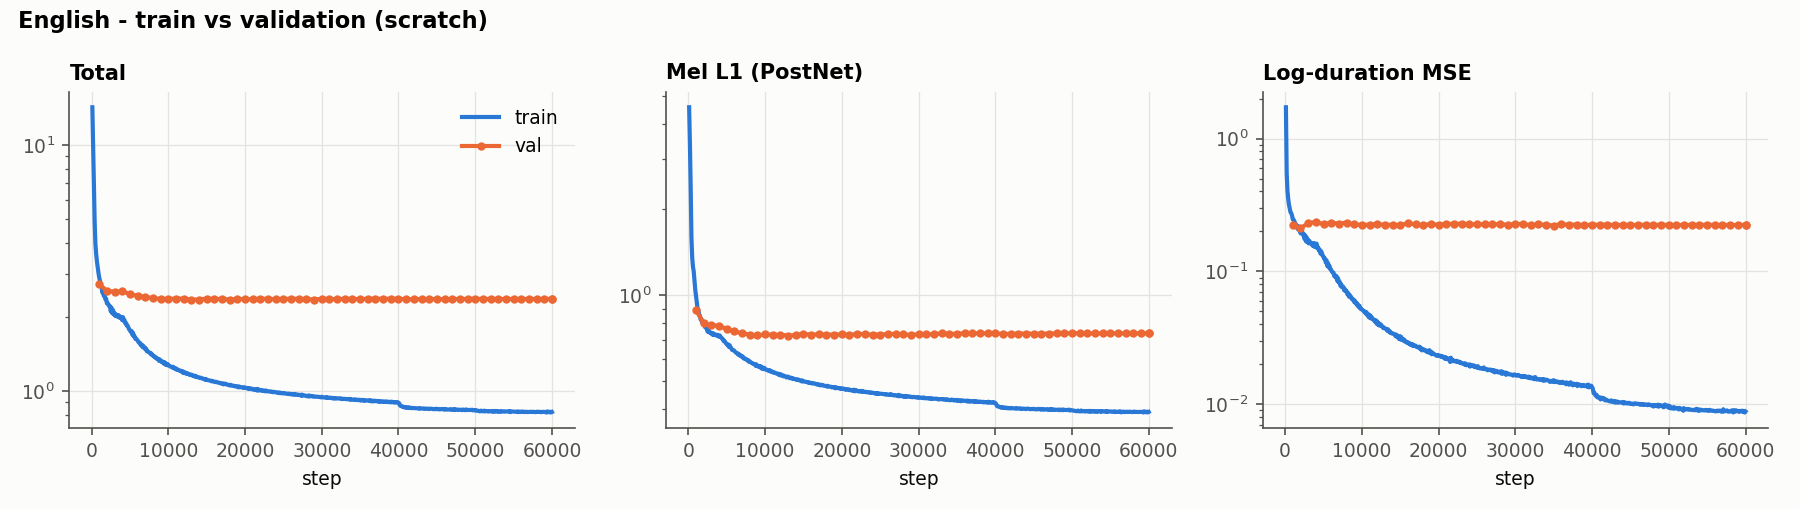
\includegraphics[width=\linewidth]{English/train_vs_val.png}
\caption{English, from scratch: training vs validation loss (log scale). The step at 40k is the first learning-rate
drop.}
\label{fig:en-trainval}
\end{figure}

\begin{figure}[H]\centering
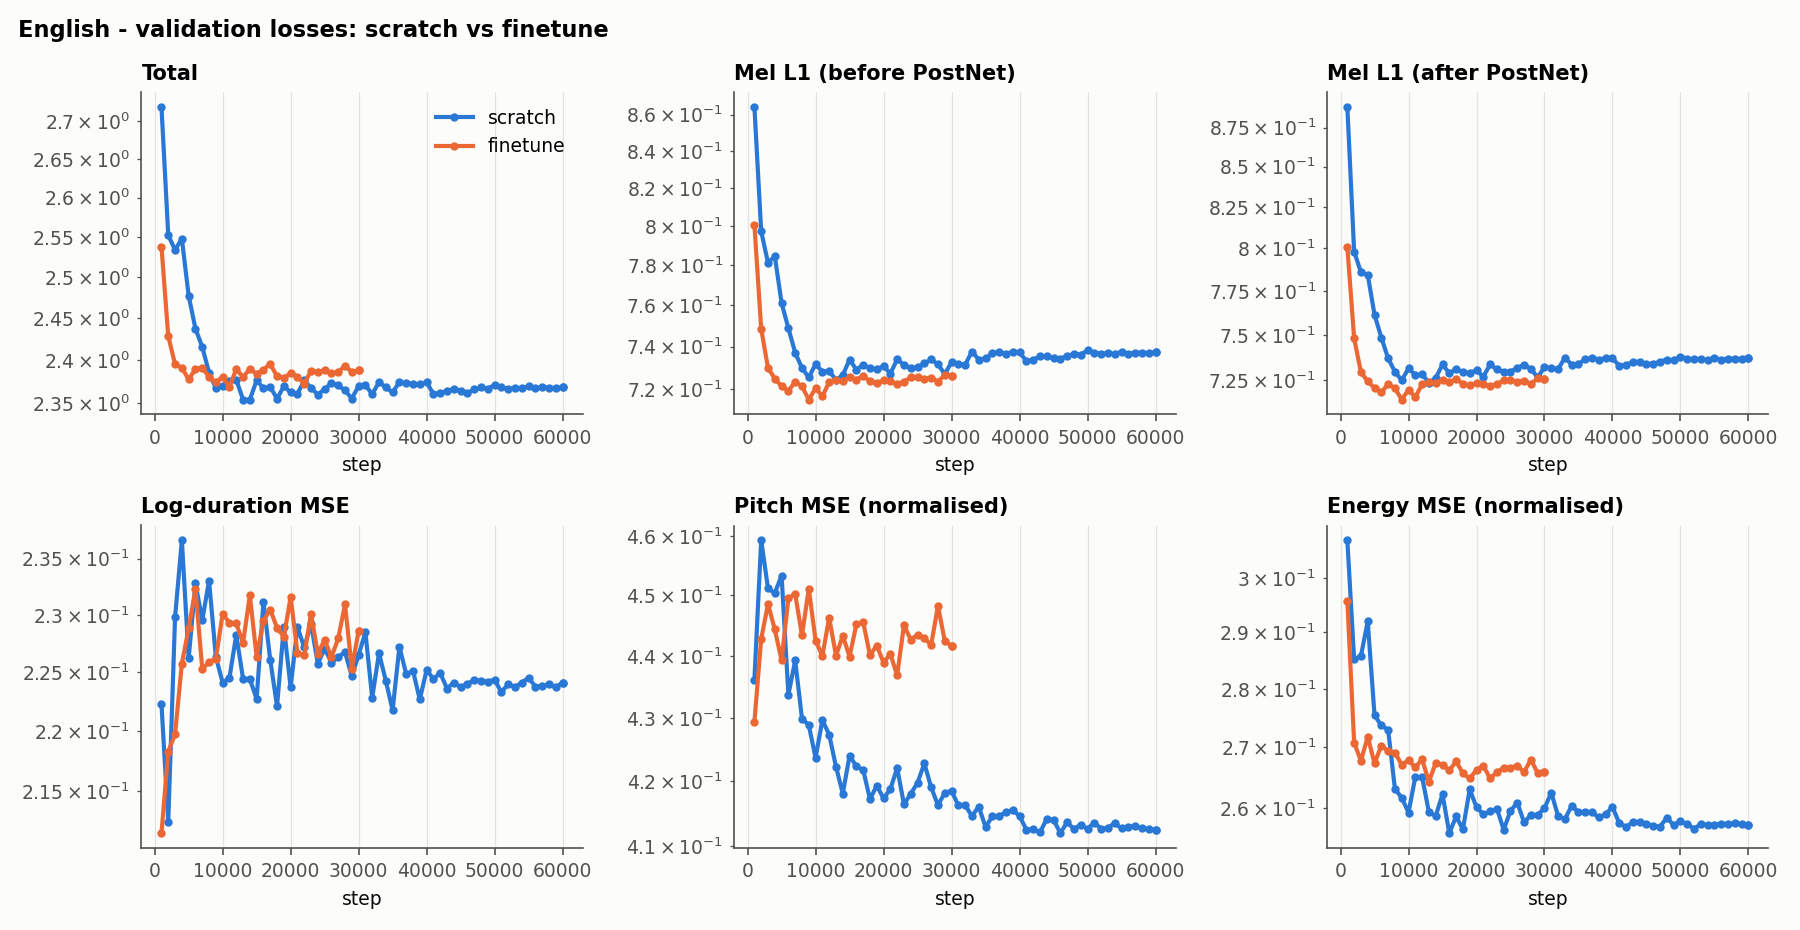
\includegraphics[width=\linewidth]{English/compare_runs_validation.png}
\caption{English validation losses, from scratch vs fine-tuned from LJSpeech.}
\label{fig:en-compare}
\end{figure}

\begin{figure}[H]\centering
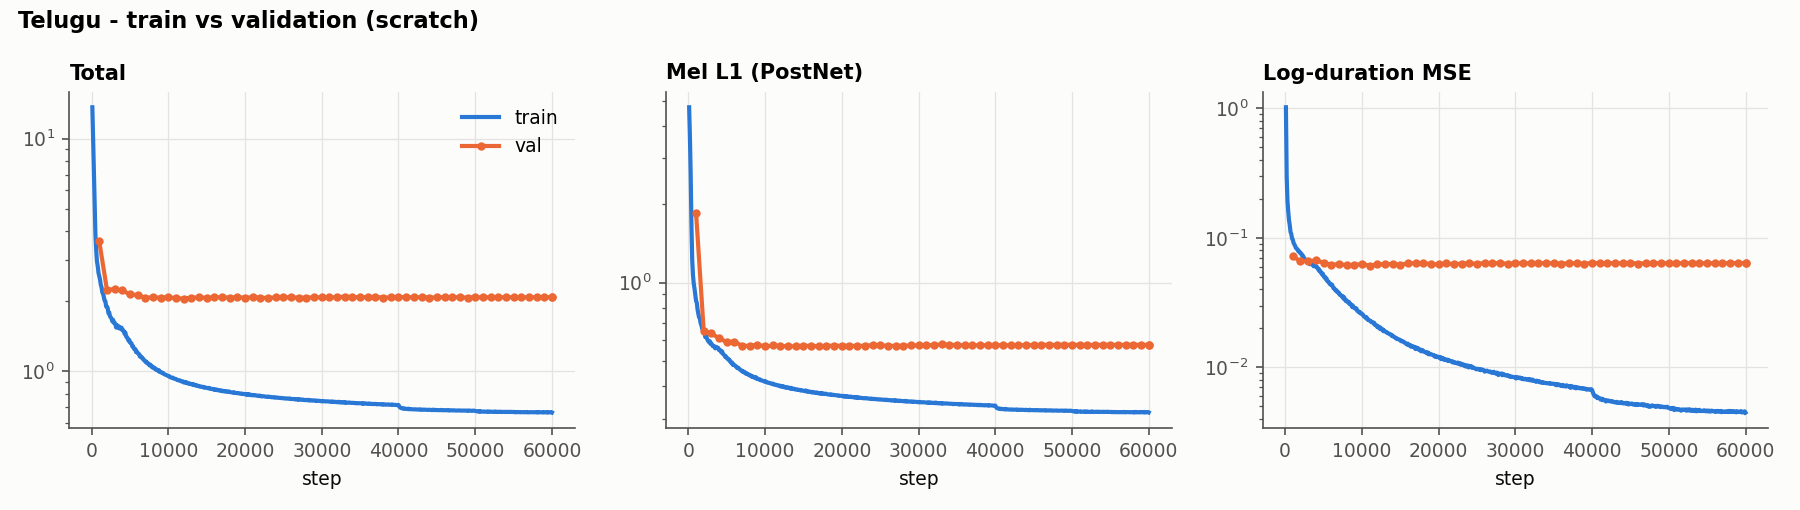
\includegraphics[width=\linewidth]{Telugu/train_vs_val.png}
\caption{Telugu: training vs validation loss (log scale).}
\label{fig:te-trainval}
\end{figure}

\paragraph{Both models stop generalising early.} English validation loss falls from 2.72 at step 1,000 to its
minimum of 2.354 at step 14,000. Over the remaining 46,000 steps it stays between 2.36 and 2.38, while the training
loss keeps falling from 1.13 to 0.82. Telugu follows the same pattern two thousand steps sooner: validation reaches
2.048 at step 12,000 and then holds between 2.06 and 2.09, while training falls from 0.89 to 0.66. In both languages
the last 46,000--48,000 steps fitted the training clips without helping on new ones: the model overfitted. The released checkpoints come
from the best steps, so they do not suffer, but three quarters of the GPU time bought nothing.

\paragraph{The loss terms move differently.} English validation mel L1 bottoms out at step 13,000 (0.724) and then
creeps up to 0.737: the decoder overfits. Validation pitch MSE keeps improving slowly until about step 46,000
(0.436 $\rightarrow$ 0.412), and energy flattens after step 16,000 at 0.256. Validation duration MSE reaches its
best at step 2,000 (0.212) and never improves again, while the training duration loss falls to 0.009. The duration
predictor learns average phone lengths almost at once and then memorises the training clips. Telugu's mel L1 also
bottoms out early (step 10,000, 0.568), but its duration and pitch keep learning longer: their validation losses
reach their minimum at steps 11,000 (0.061) and 12,000 (0.567) and then get worse, pitch up to 0.588 by the end.
Only Telugu energy improves slowly until step 38,000.

\paragraph{The gap between training and validation is large.} It is largest for English duration (0.009 vs
0.224) and pitch (0.016 vs 0.413). Three causes are likely. The data is small: 4.6\,h, split over 99 speakers, about
3\,min each. Part of Svarah is spontaneous speech, whose timing and intonation vary in ways the phones cannot
predict. Unseen voices are not the cause: validation uses the same 99 speakers as training.

\paragraph{Telugu learns duration far better, and pitch only looks worse.} Duration loss is not standardised, so
the two languages compare directly: Telugu reaches 0.061 and English 0.212. The loss is a squared error on log
durations, so its square root is a typical error on the log scale, $\sqrt{0.061}\approx0.25$ and
$\sqrt{0.212}\approx0.46$: a predicted duration is typically off by a factor of $e^{0.25}\approx1.28$ in Telugu
against $e^{0.46}\approx1.59$ in English. One voice reading prepared text times its speech
far more regularly than 99 speakers partly talking freely. Telugu's validation pitch MSE (0.567) exceeds English's
(0.418), but each corpus standardises pitch with its own spread. The English spread of 56.8\,Hz includes the
differences between 99 voices, which the speaker embedding explains for free. In Hz the root-mean-square error is
$\sqrt{0.567}\times42.7\approx32$\,Hz for Telugu and $\sqrt{0.418}\times56.8\approx37$\,Hz for English.

\paragraph{Fine-tuning from LJSpeech helps the decoder only.} The fine-tuned model starts much lower (validation
total 2.54 vs 2.72 at step 1,000) and reaches a slightly lower mel loss (best 0.715 vs 0.724). Its pitch and energy
losses stay higher, though: 0.440 vs 0.418 and 0.267 vs 0.259 at each run's best step. Its best total, 2.369, does
not beat training from scratch (2.354). The LJSpeech start gives the decoder spectral detail, but the duration, pitch and
energy predictors gain nothing. Their bins restart from zero, and one American woman reading books does not prosodically
resemble 99 Indian speakers.

% =====================================================================
\section{Test sentences}
\label{sec:test}
The audio sits in \code{Results/<Language>/test\_generated\_audios/}. Next to the plots, a JSON file per sentence
records the phones the model received and the duration, F0 and energy it predicted for each.

\paragraph{English} (released model, speaker \code{en\_s073}, male).

\begin{table}[H]\centering\small
\caption{English test sentences and what the front-end did with the hard part. Phones are in ARPAbet and come
from the saved JSON files; the digit after a vowel marks stress (1 primary, 2 secondary, 0 none).}
\label{tab:en-test}
\begin{tabularx}{\linewidth}{@{}l>{\raggedright\arraybackslash}Xr@{}}
\toprule
Id & Sentence and front-end output & Length \\
\midrule
E1 & The antidisestablishmentarianism movement gained considerable momentum during the parliamentary proceedings.
The LibriSpeech lexicon lacks the long word, but CMUdict has it: 28 phones
(\code{AE2 N T AY0 D IH0 S AH0 S T AE2 B L IH0 SH M AH0 N T EH1 R IY0 AH0 N IH0 Z AH0 M}), spoken in 1.75\,s. & 5.34\,s \\
E2a & The orchestra's conduct during the ceremony was praised by the audience. Noun: \code{K AA1 N D AH0 K T},
stress on the first syllable. & 3.41\,s \\
E2b & The researchers will conduct an experiment to evaluate the proposed method. Verb: \code{K AA0 N D AH1 K T},
stress on the second syllable. The part-of-speech tag tells the two readings apart. & 3.63\,s \\
E3 & The rhyth m of the orchestra changed unexpectedly. The repair merges ``rhyth'' + ``m'' into the dictionary
word \code{R IH1 DH AH0 M}. Without it (\code{E3\_no\_repair}) the model receives \code{R AY1 DH} + \code{EH1 M},
roughly ``rythe em''. & 2.35\,s \\
E4 & The meeting will start at 10:45 AM on 12 November 2026, so andaroo should arrive on time. The normaliser
produced ``ten forty five AM on twelfth November twenty twenty six'' and spelled AM out (\code{EY1 EH1 M}).
``Andaroo'' (Telugu for ``everyone'') went to g2p\_en, which ended it with ``oh'' instead of ``oo''
(\code{AE0 N D AA1 R OW0}). & 5.91\,s \\
\bottomrule
\end{tabularx}
\end{table}

\paragraph{The English audio sounds mumbled.} The speech is understandable and the sentences come out whole, but
the speaker seems to swallow the words: consonants are soft and syllables run into each other. FastSpeech 2 cannot
skip or repeat words, because its durations are explicit. Attention-based models such as Tacotron 2 learn the
timing implicitly and sometimes do skip or repeat. In the whole test set
only one phone received zero frames, the schwa (the weak ``uh'' vowel) of ``-able'' in ``considerable'' (\code{B AH0 L}), which speakers
often drop as well because the /l/ carries the syllable. Section~\ref{sec:var} measures the mumbling and traces it
to over-smoothed spectrograms from the decoder.

\paragraph{Telugu} (released model, one male voice). The phones use the front-end's romanisation: doubled vowels
are long, and \code{tt}, \code{dd}, \code{nn} are retroflex.

\begin{table}[H]\centering\small
\caption{Telugu test sentences and what the front-end did with the hard part.}
\label{tab:te-test}
\begin{tabularx}{\linewidth}{@{}l>{\raggedright\arraybackslash}Xr@{}}
\toprule
Id & Sentence, meaning and front-end output & Length \\
\midrule
T1 & \tel{న్యూరోఫార్మకోలాజికల్ పరిశోధనలో నూతన ఔషధాల ప్రభావాన్ని విశ్లేషించారు.} (``The effect of new drugs was
analysed in neuropharmacological research.'') The long loanword became 19 phones
(\code{n y uu r oo ph aa r m a k oo l aa j i k a l}), spoken in 1.49\,s. The G2P reads \tel{ఫ} as aspirated
\code{ph}, its textbook value, although many speakers say /f/ in English loanwords. & 4.42\,s \\
T2a & \tel{తాడుపై అతని పట్టు చాలా బలంగా ఉంది.} (``His grip on the rope is very strong.'') & 2.03\,s \\
T2b & \tel{ఆమె పట్టు చీరను ధరించి వేడుకకు వచ్చింది.} (``She came to the ceremony in a silk sari.'')
\tel{పట్టు} means ``grip'' in T2a and ``silk'' in T2b, but Telugu pronounces both the same way, so the identical
phones (\code{p a tt tt u}) are correct. & 2.38\,s \\
T3 & \tel{పులి అడ విలో నిశ్శబ్దంగా నడిచింది.} (``The tiger walked silently in the forest.'') The input splits
\tel{అడవిలో} into \tel{అడ} + \tel{విలో}, and the repair merges it again. The merge changes nothing: the G2P maps each
akshara on its own and adds no pause between words, so both versions give the phones \code{a dd a v i l oo} and
byte-identical audio. A split word costs nothing in Telugu's phonemic script. & 1.73\,s \\
T4 & \tel{ఈ సమావేశం 2026 నవంబర్ 12వ తేదీ ఉదయం 10:45 గంటలకు ప్రారంభమవుతుంది, సమయానికి సిద్ధంగా ఉంచండి.}
(``This meeting starts at 10:45 a.m. on 12 November 2026; be ready on time.'') The normaliser wrote the numbers
as \tel{రెండు వేల ఇరవై ఆరు} (2026), \tel{పన్నెండవ} (12th) and \tel{పది నలభై ఐదు} (10:45). & 7.21\,s \\
\bottomrule
\end{tabularx}
\end{table}

No Telugu phone received zero frames. The anusvara (\tel{ం}) took the nasal of the following consonant, as in
speech: \code{u n d i} (\tel{ఉంది}), \code{b a l a ng g aa} (\tel{బలంగా}) and \code{ny c} in
\tel{విశ్లేషించారు}.

\paragraph{I could not judge the Telugu audio by ear,} because I do not speak Telugu. Speech recognisers listened
instead (Section~\ref{sec:asr}), and the measurements in Section~\ref{sec:var} compare the model's predictions with real
recordings of validation sentences.

\subsection{Speech recognition check}
\label{sec:asr}
Whisper base (74\,M parameters) transcribed the audio. English used \code{openai/whisper-base.en}; Telugu used
\code{vasista22/whisper-telugu-base}, a Whisper base model that IIT Madras fine-tuned on Telugu. A recogniser
makes its own errors, so I measured a ceiling first. I took 30 random validation clips per language and turned
their \emph{real} mel spectrograms into audio with the same HiFi-GAN vocoder. The released models then synthesised
the same 30 sentences from their phones, and the difference between the two error rates is what FastSpeech 2
adds. Character error rate (CER) is the main measure. Telugu words are long, so one wrong letter fails a whole
word and inflates the word error rate (WER) even for real speech.

\begin{table}[H]\centering\small
\caption{Recogniser error rates (\%). ``Real, vocoded'' is the ceiling: real spectrograms through the same vocoder.}
\label{tab:asr}
\begin{tabular}{@{}lrrrr@{}}
\toprule
 & \multicolumn{2}{c}{English} & \multicolumn{2}{c}{Telugu} \\
 & CER & WER & CER & WER \\
\midrule
Real, vocoded (30 validation clips) & 6.4 & 14.4 & 3.4 & 21.8 \\
Synthesised, same 30 sentences & 10.0 & 21.0 & 4.7 & 23.6 \\
Test sentences (English 5 + E3\_no\_repair, Telugu 5) & 26.4 & 56.9 & 3.1 & 20.0 \\
\bottomrule
\end{tabular}
\end{table}

\paragraph{Synthesised Telugu is almost as intelligible as real speech:} 4.7\% CER against 3.4\%, a gap of
1.3 points. T1, T2a and T2b came back with every letter right; in T1 the recogniser only split the loanword into
two words (\tel{న్యూరో ఫార్మకోలాజికల్}). In T4 the year and the time came back word for word (\tel{రెండు వేల ఇరవై ఆరు}, \tel{పది నలభై ఐదు}), and its
remaining differences are word splits that sound the same: \tel{పన్నెండు వ} for \tel{పన్నెండవ} (12th) and
\tel{ప్రారంభం అవుతుంది} for \tel{ప్రారంభమవుతుంది}. T3 holds the one real error: \tel{అడవిలో నిశ్శబ్దంగా} (``silently in the forest'') came
back as \tel{అడవిలోని శబ్దంగా}. The recogniser heard one \emph{ś} where the text has two and attached the syllable
\tel{ని} to the previous word. The duration predictor did not shorten the doubled consonant: it gave the two
\emph{ś} phones 105 and 93\,ms, the longest consonant in the sentence. Either the vocoded audio blurs the double
\emph{ś}, or the recogniser preferred a more common word split; the data here cannot tell which.

\paragraph{Synthesised English loses more:} 10.0\% CER against 6.4\% for real speech, 3.6 points, and 21.0\%
against 14.4\% WER. On 30 clips this gap only approaches significance (Section~\ref{sec:ablation}). The larger
gap matches the flux measurement in Table~\ref{tab:var} and the mumbled sound.
The test sentences fare far worse (26.4\% CER), because they are built from rare words that a 74\,M recogniser
struggles with even when spoken clearly. I have no real recordings of them, so the table cannot separate the two
causes. E2a came back almost perfectly, with only ``audience'' heard as ``Indians''. E1 became ``the untetish
establishment, the Zionism movement'', and ``momentum'' became ``movement''. In E2b the opening ``The researchers
will conduct an'' became ``Please suggest welcome the pen''. E4 kept the time (``10.45'') but lost ``AM'', the date and ``so andaroo''. In
E3 the recogniser heard ``I don't know if'' for ``The rhythm of'' and scored the repaired version (39.6\% CER)
worse than the unrepaired one (16.7\%). One sentence through one recogniser cannot show whether the repair helps;
the phones in Table~\ref{tab:en-test} show that it gives the model the right input.

\paragraph{Scoring details.} Svarah writes numbers as words and Whisper writes digits, so Whisper's English
normaliser maps both sides to digits before scoring. Whisper's basic normaliser cannot score Telugu: it deletes
Unicode combining marks, which in Telugu are the vowel signs and the virama, and would compare bare consonants. For
Telugu I removed only punctuation. I also raised the output limit to 440 tokens, because Telugu needs many tokens
per word and the default cut long sentences short. \code{Results/<Language>/logs/asr\_check.json} holds every
transcript, and \code{tools/} holds the scripts.

% =====================================================================
\section{Variance adaptor predictions}
\label{sec:var}
The variance adaptor predicts each phone's duration, pitch and energy (Section~\ref{sec:background}). Every test
sentence has four plots of its predictions in \code{Results/<Language>/variance\_adaptor\_plots/}: predicted duration per
phone, F0 per phone in Hz, energy per phone, and an overview that stacks the generated mel spectrogram over F0 and
energy on one time axis (Figures~\ref{fig:en-ov} and~\ref{fig:te-ov}).

\begin{figure}[H]\centering
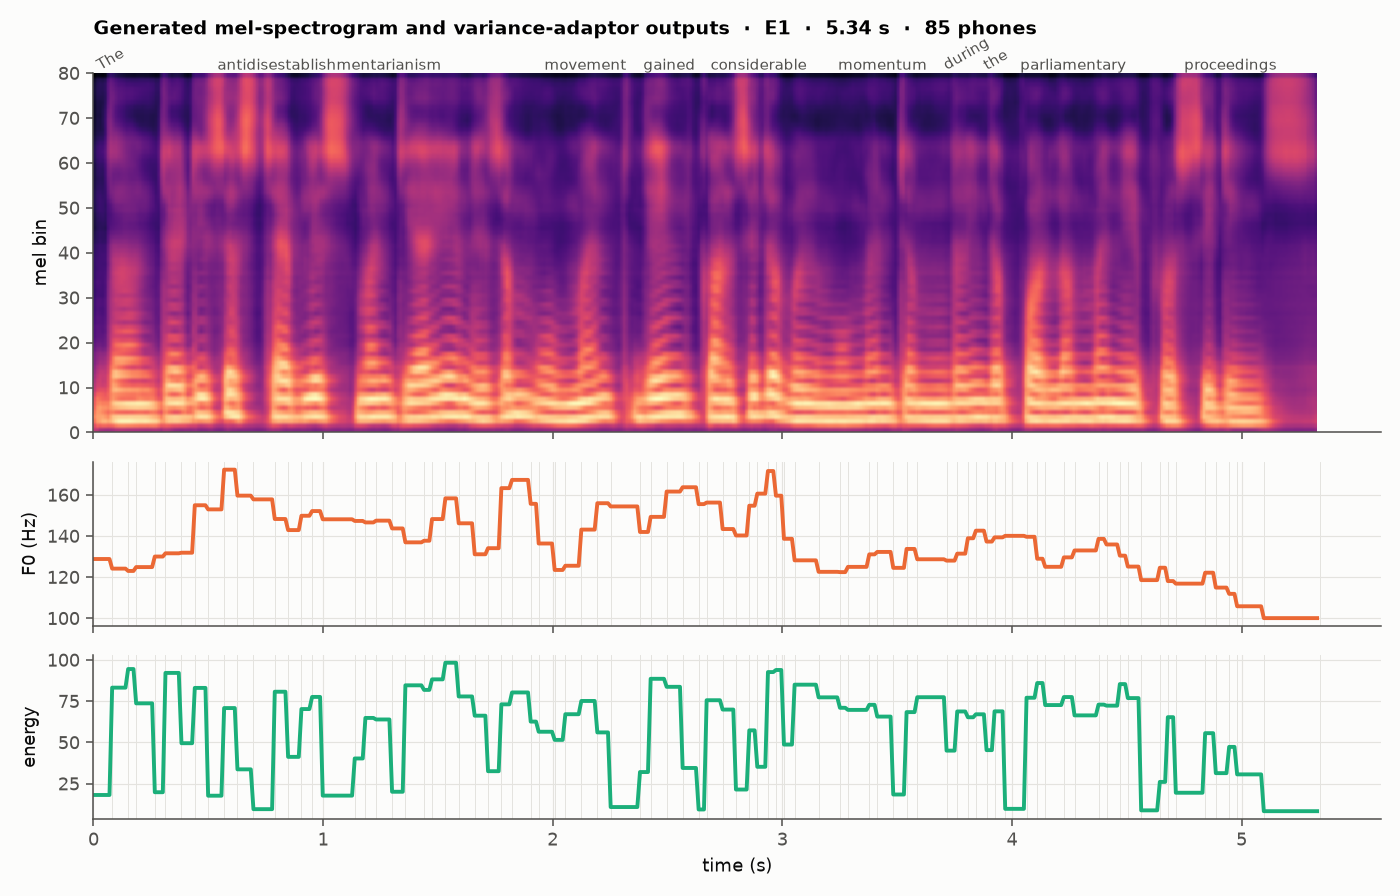
\includegraphics[width=0.92\linewidth]{English/variance_adaptor_plots/overview/E1.png}
\caption{English E1. Top: the generated mel spectrogram (bright means loud; low bands at the bottom), with the
words above. Middle and bottom: the predicted F0 and energy of each phone; thin vertical lines mark phone
boundaries. Energy is the STFT frame norm, in arbitrary units.}
\label{fig:en-ov}
\end{figure}

\begin{figure}[H]\centering
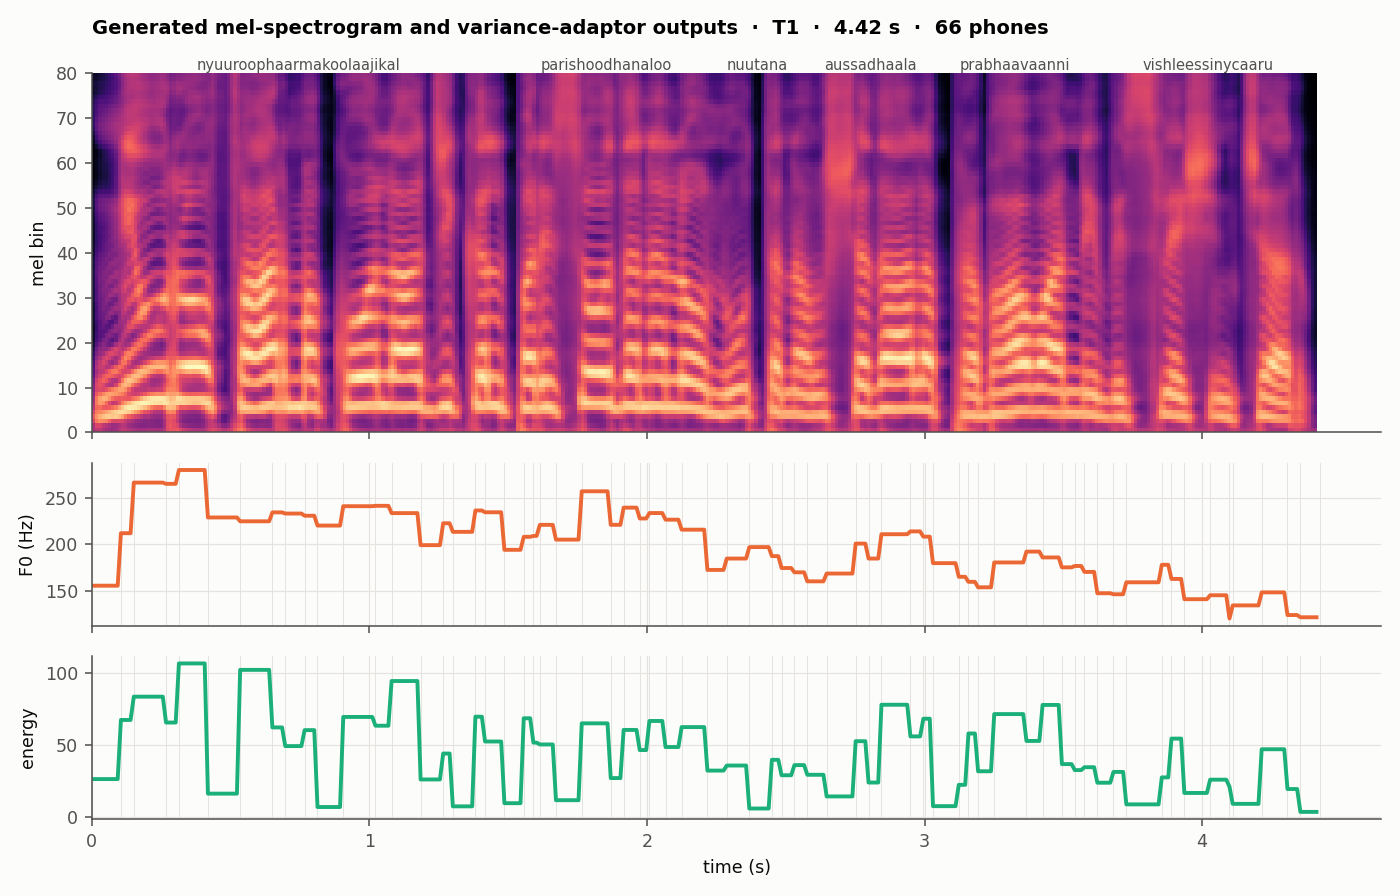
\includegraphics[width=0.92\linewidth]{Telugu/variance_adaptor_plots/overview/T1.png}
\caption{Telugu T1, laid out like Figure~\ref{fig:en-ov}. The plotting library cannot draw Telugu script, so the
word labels show the romanised phones.}
\label{fig:te-ov}
\end{figure}

\subsection{Against real speech}
Test sentences have no recording to compare with, so I ran the released models on 80 random validation clips per
language and compared each prediction with the real features of the same clip. The model received the clip's
phones, including the pauses that MFA found, and predicted everything else itself. Predicted and real durations
differ, so I compare utterance-level statistics, not frames.

\begin{table}[H]\centering\small
\caption{Predictions on 80 validation clips per language against the real features of the same clips (medians).
For every row, 1.0 means a perfect match. A spread ratio is predicted / real standard deviation within an
utterance. Global variance is each mel band's variance over the utterance; flux is the mean absolute change between
neighbouring frames (Table~\ref{tab:terms}).}
\label{tab:var}
\begin{tabular}{@{}lccc@{}}
\toprule
 & English & English fine-tuned & Telugu \\
\midrule
Pitch spread ratio & 0.67 & 0.75 & 0.85 \\
Energy spread ratio & 0.96 & 0.98 & 0.94 \\
Pitch correlation (per phone) & 0.43 & 0.39 & 0.75 \\
Energy correlation (per phone) & 0.82 & 0.82 & 0.92 \\
Log-duration correlation (per phone) & 0.61 & 0.61 & 0.85 \\
Predicted / real length & 0.96 & 0.99 & 0.97 \\
Mel global variance, predicted / real & 0.85 & 0.88 & 0.97 \\
Mel flux, predicted / real & 0.63 & 0.61 & 0.88 \\
\bottomrule
\end{tabular}
\end{table}

\paragraph{Flux measures the mumbling.} A real English spectrogram changes from one frame to the next 1.6 times as
much as the predicted one (flux ratio 0.63). Transitions between sounds therefore blur: the burst of a /t/ or /k/, the jump
from consonant to vowel, the movement of a formant (a resonance of the mouth that identifies a vowel). That is what ``swallowed'' words sound like. The L1 mel loss
causes it. When several spectrograms fit the same phones, the loss rewards their middle, and the middle of several
sharp transitions is one soft one. Telugu loses much less (0.88), because one speaker's read speech leaves fewer
plausible spectrograms to average. The fine-tune keeps more overall variance (0.88) but not sharper transitions
(0.61); LJSpeech gave the decoder detail, not crispness.

\paragraph{Intonation comes out flat in English.} The English model's pitch varies two thirds as much as the real
pitch inside an utterance (0.67), and follows its shape only loosely ($r = 0.43$). Averaging explains the
flatness again: when the text does not decide whether a phrase rises or falls, the safest prediction stays near the
mean. Telugu keeps 85\% of the real spread and tracks the contour well ($r = 0.75$). Energy follows the real values
closely in both languages ($r = 0.82$ and 0.92) with nearly the right spread, because energy depends mostly on
which phone is spoken: vowels are loud and stops quiet.

\paragraph{Both models speak slightly fast.} Given the same phones, they produce 3--4\% less time than the real
speaker took. The duration correlation repeats the loss curves: 0.85 for Telugu, 0.61 for English.

\subsection{Which prediction costs the most?}
\label{sec:ablation}
Table~\ref{tab:var} shows how the predictions differ from real speech, not what each difference costs. To measure
that, I gave the released models the real values from the recording in place of their own predictions, one part
at a time, on the same 30 validation clips as Section~\ref{sec:asr}. Every version went through the same HiFi-GAN
and the same recogniser. Two further measures compare each version with the real recording: mel-cepstral
distortion (MCD), the distance between the generated and the real spectrogram, and the root-mean-square F0 error
in cents (100 cents make a semitone). Lower is better for both (Table~\ref{tab:terms}).

\begin{table}[H]\centering\small
\caption{Real values in place of predictions, on 30 validation clips per language (means; lower is better in
every column). Each row names what the model was given from the recording instead of predicting it. ``Real
recording, vocoded'' is the recording's own spectrogram through the vocoder; MCD and F0 error use it as the
reference.}
\label{tab:ablation}
\begin{tabular}{@{}lrrrrrr@{}}
\toprule
 & \multicolumn{3}{c}{English} & \multicolumn{3}{c}{Telugu} \\
\cmidrule(lr){2-4}\cmidrule(l){5-7}
Taken from the recording & CER \% & MCD dB & F0 cents & CER \% & MCD dB & F0 cents \\
\midrule
Nothing (the normal system) & 10.0 & 3.05 & 310 & 4.7 & 2.55 & 316 \\
Durations & 12.3 & 3.05 & 302 & 3.8 & 2.50 & 298 \\
Pitch and energy & 10.0 & 2.78 & 202 & 3.7 & 2.04 & 119 \\
Durations, pitch and energy & 11.5 & 2.81 & 180 & 4.2 & 1.98 & 116 \\
\midrule
Real recording, vocoded & 6.4 & -- & -- & 3.4 & -- & -- \\
\bottomrule
\end{tabular}
\end{table}

\paragraph{Pitch and energy cost the most; durations cost almost nothing.} Real pitch and energy cut MCD by
0.27\,dB in English (9\%) and 0.51\,dB in Telugu (20\%), and the F0 error by 108 and 198 cents. Real durations
moved MCD by 0.00 and 0.05\,dB and the F0 error by 8 and 18 cents. A paired bootstrap over the 30 clips (5,000
resamples) puts the pitch-and-energy gains far from zero: the 95\% interval for the English MCD gain runs from
0.18 to 0.36\,dB. The duration gains stay within 0.1\,dB of zero in both languages. The English duration
predictor's weak correlation ($r = 0.61$) therefore costs little: with the real timing, the decoder makes
spectrograms of the same quality.

\paragraph{The English decoder sets the floor.} With every prosody value taken from the recording, English still
reaches only 2.81\,dB, against 1.98\,dB for Telugu. What remains comes from the decoder, the part that turns phones
and prosody into a spectrogram. Real prosody does not close the gap between the languages; it widens it, from
0.50\,dB with predictions to 0.83\,dB with real values, because Telugu gains more from real pitch than English
does. The mumbled English sound therefore comes from the decoder, not from the timing, and real durations do not
remove it. The first two improvements in Section~\ref{sec:cmp} target exactly this part.

\paragraph{Pitch stays off even when it is real.} With the real pitch, the F0 error still comes to 180 cents in
English and 116 in Telugu. The model receives one pitch value per phone, so it cannot reproduce the rise or fall
inside a phone. English adds noisier recordings, which make F0 harder to extract on both sides: even with
everything real, the generated and the real audio disagree on whether a frame is voiced in 22\% of English frames
against 13\% of Telugu frames.

\paragraph{The recogniser cannot separate the versions.} No English version differs from the normal system by
more than the noise: every 95\% interval spans zero and covers 6 to 7 points. In Telugu, real pitch and energy
lowered CER by 1.1 points (interval 0.2 to 2.0), but with real durations added the gain shrank to 0.5 and lost
significance, so I read no pattern into it. Thirty clips can resolve a difference of about 1 point in Telugu and
only about 3 in English. The same caution applies to Table~\ref{tab:asr}. Telugu's 1.3-point gap between real and
synthesised speech holds (interval 0.3 to 2.5), but English's 3.6-point gap does not quite (interval $-0.4$ to 7.3).

\paragraph{Method details.} MCD uses cepstral coefficients 1 to 24 of the 80-band log-mel spectrogram, averaged
over DTW-aligned frames, silences included. It compares the model's spectrogram before the vocoder. Other papers
usually compute MCD from WORLD or SPTK spectral envelopes, so these absolute values compare versions within this
report, not with published numbers. I aligned every version with DTW, even when the lengths matched, so the
versions with real durations face the same alignment as the rest. F0 comes from WORLD (DIO with StoneMask) on the
vocoded audio, scored against the vocoded real spectrogram so that the vocoder affects both sides equally, over
frames voiced in both. \code{Results/<Language>/ablation\_samples/} holds three of the clips in all five versions
for listening, and \code{logs/ablation.json} holds every number and transcript.

\subsection{In the test sentences}
\begin{itemize}
\item \textbf{Declination.} F0 falls through every sentence, as it does in natural statements. The mean F0 of the
last third of the vowels lies below that of the first third in all ten sentences: by 15--25\,Hz in English
(for example 145 $\to$ 123\,Hz in E2a) and by 16--74\,Hz in Telugu (236 $\to$ 163\,Hz in T1).
\item \textbf{Pauses at commas.} E4 and T4 each contain a comma, and the front-end turns it into a pause token.
The duration predictor gave those pauses 360\,ms (E4) and 314\,ms (T4), a natural length for a clause break. The
other eight sentences have no internal punctuation and got no pauses.
\item \textbf{Stress in ``conduct'' (E2a vs E2b).} The model marks the first syllable as the heteronym table
intends. Stressed in the noun, its vowel lasts 58\,ms at 139\,Hz with energy 73; unstressed in the verb, it lasts
35\,ms at 133\,Hz with energy 56. The second syllable follows only in loudness: the verb's stressed \code{AH1} is
louder than the noun's unstressed \code{AH0} (76 vs 68), but shorter (46 vs 93\,ms) and lower (120 vs 130\,Hz).
The model has learnt the stress contrast on the first syllable and only part of it on the second.
\item \textbf{Final lengthening appears in four sentences of ten.} The last word's vowels last longer than the
sentence's average vowel in E3, E4, T2a and T4 (for example 104 vs 60\,ms in E4), but not in the other six.
\item \textbf{Speaking rate} lies between 14.2 and 15.9 phones per second in English and between 14.9 and 17.9 in
Telugu.
\end{itemize}

% =====================================================================
\section{English vs Telugu, limitations and improvements}
\label{sec:cmp}
\paragraph{Telugu wins on every measure.} Telugu has a lower validation loss (2.048 vs 2.354), better duration and
pitch tracking (Table~\ref{tab:var}), spectrograms closer to real speech in both variance and flux, and a smaller
intelligibility loss against real speech (1.3 vs 3.6 CER points, Table~\ref{tab:asr}). The data
explains this better than the language does. The Telugu model hears one speaker for 4.1\,h of read, studio-quality
speech. The English model hears 99 speakers for about 3 minutes each, part of it spontaneous, recorded for ASR
testing rather than synthesis. Telugu's phonemic script also helps: the rule-based G2P has no unknown words, while
English needed g2p\_en guesses for 1,158 words of its training dictionary and for ``andaroo'' at test time.

\paragraph{Limitations.}
\begin{itemize}
\item \textbf{Over-smoothed English spectrograms} (flux ratio 0.63) make the speech sound mumbled. The decoder
causes this, not the prosody predictions (Section~\ref{sec:ablation}).
\item \textbf{Flat English intonation} (pitch spread ratio 0.67, $r = 0.43$).
\item \textbf{Wasted training:} both models peaked by step 14,000 of 60,000.
\item \textbf{Speaker identity in English rests on a guess:} 115 metadata groups for 117 real speakers.
\item \textbf{Loanwords:} the Telugu G2P reads \tel{ఫ} as \code{ph} where speakers often say /f/, and the English
front-end mispronounces Telugu words such as ``andaroo''.
\item \textbf{One pitch value per phone} cannot express a rise or fall inside a long vowel.
\item \textbf{No listening test:} English quality rests on my own listening, and Telugu quality on a speech
recogniser and the measures in Table~\ref{tab:var}, because I do not speak Telugu. A recogniser measures whether
words survive, not whether speech sounds natural. A mean opinion score (MOS), in which several native listeners of each language
rate naturalness from 1 to 5, would settle both.
\end{itemize}

\paragraph{Improvements, in the order I would try them.}
\begin{enumerate}
\item \textbf{Fine-tune HiFi-GAN on this model's outputs.} Running the trained FastSpeech 2 with the real durations
gives predicted mels aligned to real audio; training the vocoder on those pairs teaches it to restore the detail
FastSpeech 2 smooths away. The HiFi-GAN authors fine-tune their vocoder on the outputs of Tacotron 2 in the
same way. This attacks
the mumbling directly and needs no new data.
\item \textbf{Add an adversarial loss on the mel spectrogram.} A second network, a discriminator, learns to tell generated from real spectrograms and so penalises the
averaged, blurred spectrograms that L1 rewards; this targets the flux deficit in Table~\ref{tab:var}.
\item \textbf{Give English fewer speakers with more audio each}, for example the 20 speakers with the most clean
read speech. Three minutes per voice is too little to learn a voice's timing and intonation.
\item \textbf{Stop early.} Ending a run once validation loss has not improved for 10,000 steps would have cut
training to about 24,000 steps, 40\% of the GPU time.
\item \textbf{Fine-tune from LJSpeech with a truly low learning rate} (peak around $10^{-4}$), so that the
pretrained decoder keeps what it knows.
\item \textbf{Add loanword rules}: \tel{ఫ} $\to$ /f/ in recognised English loanwords, and a Telugu-to-ARPAbet
mapping for Telugu words in English text.
\end{enumerate}

% =====================================================================
\section{Changes to the reference code}
\label{sec:changes}
This section lists every change to \code{ming024/FastSpeech2}, as the assignment asks. The repository keeps the
ming024 file layout under \code{core/}.

\subsection*{Bug fixes and updates}
\begin{enumerate}
\item \textbf{Silences in MFA 2/3 TextGrids.} MFA 2 and 3 write silences as empty intervals, and \code{tgt}, the library
that reads TextGrid files, drops empty intervals by default. The phone durations then no longer added up to the mel length, which shifted every
phone after a pause. The reader now keeps empty intervals and turns them into the pause phone \code{sp}
(\code{include\_empty\_intervals=True}); it skips utterances that contain \code{spn}, MFA's mark for a word it
could not align.
\item \textbf{Energy control.} The pitch control (\code{p\_control}) scaled the energy predictor; the energy control
(\code{e\_control}) now does.
\item \textbf{Energy targets in float64.} ming024's \code{to\_device} converts every target to 32-bit floats
(float32) except energy, and the energy files hold 64-bit floats (float64). Plain fp32 training on a CPU tolerates this. Under mixed precision on
the GPU the backward pass fails (\code{Found dtype Double but expected Float}); both first Kaggle runs crashed on it. Energy
now goes through \code{.float()}, and the loss casts every target to the prediction's type.
\item \textbf{CPU and worker processes.} The STFT called \code{.cuda()} unconditionally, which broke CPU runs and
forked feature-extraction workers. It now runs on the input's device.
\item \textbf{librosa $\geq$ 0.10.} \code{pad\_center} and \code{mel} need keyword arguments.
\item \textbf{Length regulator} vectorised with \code{torch.repeat\_interleave}: same output, faster on GPU.
\item \textbf{All-zero predicted durations} now still produce one frame.
\item \textbf{Checkpoints} store the learning rate as a plain float, so
\code{torch.load(weights\_only=True)} can read them.
\end{enumerate}

\subsection*{Additions}
\begin{enumerate}[resume]
\item \code{lr\_scale} in the scheduler and \code{--init\_from} in training, for fine-tuning. Every tensor with a
matching shape is copied; the phone embedding copies its overlapping rows; the pitch and energy bins come from the
new data; new tensors such as the speaker table keep their random start.
\item A split file written at data selection fixes the train/validation lists, instead of a random shuffle.
\item Feature extraction runs in parallel, and each language and voice sets its own F0 search range.
\item Training: mixed precision (fp16 autocast), a full validation pass every 1,000 steps, all losses in a CSV
file, best (lowest validation loss) and last checkpoints, \code{--resume}, and a wall-clock budget for Kaggle.
\item Inference: language-specific text front-ends (Section~\ref{sec:frontends}). Each sentence gets a JSON file with the predicted duration
(frames and ms), F0 (Hz) and energy per phone, de-normalised with the corpus statistics, and four plots.
\item \textbf{Telugu support}, which the reference code lacks: a text normaliser and a rule-based G2P
(Section~\ref{sec:te-frontend}), and a Telugu MFA acoustic model trained on the selected corpus, because MFA has no
pretrained one. The 49 Telugu phones go at the \emph{end} of the symbol table, the list that maps each phone to the
number the model reads, so the original symbols keep their numbers and the LJSpeech checkpoint still loads.
\item \textbf{English front-end}: number, date and time normalisation and a split-word repair
(Section~\ref{sec:en-frontend}).
\item Data preparation scripts for both corpora (selection, quality filters, split), and a script that builds
self-contained Kaggle notebooks.
\end{enumerate}

% =====================================================================
\section{Reproducibility}
\label{sec:repro}
\paragraph{Software.} Python 3.11 for data preparation and 3.13 on Kaggle; PyTorch 2.11 with CUDA 12.8 on Kaggle
and a CPU build for data preparation; librosa 0.11; pyworld; soundfile; soxr; tgt; g2p\_en 2.1.0 with NLTK
(\code{averaged\_perceptron\_tagger(\_eng)}, \code{cmudict}); inflect; pandas; pyarrow; matplotlib.
\code{requirements.txt} lists them all. Montreal Forced Aligner 3.4.3 runs in its own conda environment
(\code{core/prep/mfa.sh setup}). Its PostgreSQL server refuses to run as root, so the script runs MFA as an
unprivileged user \code{mfa}. MFA 3.4 has no \code{--beam} flag, so the beams go through a YAML file.

\paragraph{Configuration.} \code{English/config.yaml} and \code{Telugu/config.yaml} hold everything that affects
the results: selection thresholds, feature settings, model size, optimiser and steps. The Kaggle preparation step also saves the
copy it used (\code{config\_used.yaml}) next to the prepared data. \code{split.tsv} fixes the data split, and seed 1234 fixes
selection and training. GPU training still differs slightly between runs, because some CUDA kernels are
non-deterministic and fp16 rounds differently. Inference does reproduce: I cloned the public repository into
an empty folder, followed the README, and ran every inference command on CPU. The English test audio came out
identical to the released files byte for byte (I made those on CPU too). The Telugu files came from the Kaggle GPU,
and the CPU rerun matched their predicted pitch within 0.11\,Hz and their durations exactly, except for one phone of
T2b that lost a single frame (12\,ms).

\paragraph{Commands.} From the repository root (\code{README.md} has the same commands with comments). The
data preparation steps run as root, because of MFA's \code{mfa} user:
\begin{verbatim}
pip install -r requirements.txt
python -c "import nltk; [nltk.download(r) for r in ['averaged_perceptron_tagger',
           'averaged_perceptron_tagger_eng', 'cmudict']]"
curl -L -o core/hifigan/generator_universal.pth.tar.zip \
 https://github.com/ming024/FastSpeech2/raw/master/hifigan/generator_universal.pth.tar.zip
bash core/prep/mfa.sh setup                  # MFA 3.4.3 (+ user "mfa")
# data selection -> MFA alignment -> features (as root)
python English/preprocess.py --stage all --hf_dir <svarah parquet dir>
python Telugu/preprocess.py  --stage all --hf_dir <indictts parquet dir> --gender male
# training (best + last checkpoints, CSV losses in work/<Lang>/logs)
python English/train.py
python English/train.py --config English/config_finetune.yaml --tag finetune \
       --init_from <LJSpeech_900000.pth.tar> --total_step 30000
python Telugu/train.py
# test sentences -> Results/<Lang>/{test_generated_audios, variance_adaptor_plots}
python English/inference.py --speaker en_s073
python English/inference.py --speaker en_s073 --no_repair --suffix _no_repair --only E3
python English/inference.py --speaker en_s034 \
       --out_dir Results/English/other_speakers/en_s034
python English/inference.py --config English/config_finetune.yaml --speaker en_s073 \
       --ckpt English/checkpoints/finetune/best_model_fp16.pth.tar \
       --out_dir Results/English/finetune_ablation
python Telugu/inference.py
python Telugu/inference.py --no_repair --suffix _no_repair --only T3
# loss plots + fp16 release checkpoints
python core/export.py --lang English \
       --runs scratch:work/English/logs finetune:work/English/logs/finetune \
       --ckpt_dirs scratch:English/checkpoints finetune:English/checkpoints/finetune
python core/export.py --lang Telugu --runs scratch:work/Telugu/logs \
       --ckpt_dirs scratch:Telugu/checkpoints
\end{verbatim}
The Kaggle notebooks in \code{kaggle/} run the same commands, and \code{kaggle/build\_notebooks.py} rebuilds them
with the current code embedded. The scripts in \code{tools/} produce every evaluation in Sections~\ref{sec:asr}
and~\ref{sec:var}, and \code{Results/<Language>/logs/} keeps their outputs: \code{asr\_eval.py} and \code{asr\_rescore.py} the recogniser check, \code{variance\_eval.py}
Table~\ref{tab:var}, and \code{ablation\_eval.py} with \code{ablation\_ci.py} Table~\ref{tab:ablation} and its
intervals. Each script's header gives its arguments. They need \code{transformers} and \code{jiwer} on top of
\code{requirements.txt}.

\paragraph{Checks.} \code{tools/sanity\_checks.py} tests four things that could go wrong without any error
message; all four passed.
\begin{itemize}
\item \textbf{Features match the audio.} In all 7,342 clips (3,136 Telugu, 4,206 English) the phone durations
add up exactly to the mel length, and pitch, energy and duration each hold one value per phone. A mismatch would
shift every feature after it, which is what the TextGrid silence bug did before the fix.
\item \textbf{The released checkpoints are the logged ones.} The training code's own validation function,
run on CPU in fp32 over the full validation set, gives 2.0482 for the Telugu fp16 checkpoint (logged 2.0481) and
2.3540 for English (logged 2.3540). Validation runs with dropout off and without gradients.
\item \textbf{The learning rate follows the schedule.} The logged values match the Noam formula with the three
drops: $2.47\times10^{-5}$ at step 100 and $6.89\times10^{-6}$ at step 60,000.
\item \textbf{The speaker table changes the voice.} Speaker \code{en\_s073} has a median F0 of 127\,Hz in the
training data and 131\,Hz in the synthesised test sentences; speaker \code{en\_s034} has 209\,Hz in both.
\end{itemize}

\paragraph{Checkpoints.} \code{<Lang>/checkpoints/best\_model\_fp16.pth.tar} holds the weights with the lowest
validation loss in fp16. At about 70\,MB each they stay under GitHub's 100\,MB file limit, so Git LFS is not needed.
The normalisation statistics, speaker map and vocabulary that inference needs sit next to each checkpoint. The
trained Telugu MFA acoustic model is in \code{Telugu/mfa\_model/}.

\end{document}
